\documentclass[12pt,twoside]{report}

% PACCHETTI FONDAMENTALI
\usepackage{amsmath,amsfonts,amssymb,amsthm, dsfont, mathtools}
\usepackage{graphicx}
\usepackage[a4paper,outer=2cm,inner=3cm,top=3.3cm,bottom=2.5cm]{geometry}
\usepackage{float} % per il comando [H] per le tabelle
\usepackage{enumerate} % per scegliere i caratteri degli elechi
\usepackage{accents}
\usepackage{esint}
% intestazione pagine
\usepackage{fancyhdr}

% NOMENCLATURA
% indice
\renewcommand*\contentsname{Contents}
% capitoli
\renewcommand{\chaptername}{Chapter}
% appendici
\renewcommand{\appendixname}{Appendices}
% bibliografia
\renewcommand\bibname{Bibliography}
    
% TITOLI
% per mettere i titoli dei capitoli sulla destra e aggiungere una riga di separazione sotto
\usepackage{titlesec} 
\newcommand*{\justifyheading}{\raggedleft}
\titleformat{\chapter}[display]
  {\normalfont\LARGE\bfseries\justifyheading}
  {\chaptertitlename\ \thechapter \vspace*{-0.5cm}}
  {20pt}{\Huge}
  [\vspace*{0.3cm}\hrule height 0.08cm \vspace*{1cm}]

% STUTTURE FONDAMENTALI
% teoremi
\theoremstyle{plain}
\newtheorem{theorem}{Theorem}[section]
% lemmi
\newtheorem{lemma}[theorem]{Lemma}
% teoremi con nomi
\newtheoremstyle{named}{}{}{\itshape}{}{\bfseries}{.}{.5em}{\thmnote{#3} #2}
\theoremstyle{named}
\newtheorem{namedtheorem}[theorem]{Theorem}
% ipotesi
\newenvironment{ipotesi}%
{\quad\left|\quad\def\arraystretch{1.2}\begin{array}{@{}l@{}}}%
{\end{array}\right.}
% tesi
\newcommand{\tesi}[1]{\quad\left|\quad{#1}\right.}
% unico comando per ipotesi e tesi
\newcommand{\hpth}[2]
{
\begin{flalign*}
\quad\quad
\text{Hypothesis}
&\begin{ipotesi}
#1
\end{ipotesi}&&\\
\quad\quad
\text{Thesis}
&\tesi{#2}&&
\end{flalign*}
}
% quando ci sono 2 tesi distinte
\newcommand{\hpthth}[3]
{
\begin{flalign*}
\quad\quad
\text{Hypothesis}
&\begin{ipotesi} 
#1
\end{ipotesi}&&\\
\quad\quad
\text{Thesis 1}
&\tesi{#2}&&\\
\quad\quad
\text{Thesis 2}
&\tesi{#3}&&
\end{flalign*}
}
% dimostrazioni
\renewcommand*{\proofname}{\bf{Proof:}}
\renewcommand\qedsymbol{\textsc{qed}}
% definizioni
\theoremstyle{definition}
\newtheorem{definition}{Definition}[section]
% esempi
\newtheorem{example}{Example}
% osservazioni
\theoremstyle{remark}
\newtheorem*{remark}{Remark}

% NOTAZIONE
% sistemi
\newenvironment{system}%
{\left\lbrace\begin{array}{@{}l@{}}}%
{\end{array}\right.}
% parte intera
\newcommand{\interior}[1]{\accentset{\circ}{#1}}
% norma
\newcommand\norm[1]{\left\lVert#1\right\rVert}
% absolute value
\newcommand\abs[1]{\left|#1\right|}

% PAGINA BIANCA
\usepackage{afterpage}
\newcommand\blankpage{%
    \null
    \thispagestyle{empty}%
    \newpage}

% ALTRI
% indentazione del testo a 0
\parindent 0px
% numerazione in align*
\newcommand\numberthis{\addtocounter{equation}{1}\tag{\theequation}}
% citazione
\usepackage{epigraph}
% immagini
\usepackage{wrapfig}




\begin{document}
% non contare la pagina del titolo
\pagenumbering{gobble}

% titolo
\thispagestyle{empty}
\newgeometry{margin=1in}

\mdseries{

\vspace*{-1.5cm}
\begin{center}
\includegraphics[width=5cm]{logo.png}

\vspace*{0.6cm}
{\LARGE\textsc{Politecnico di Milano}}\\
\rule{8.5cm}{1pt}

\vspace*{0.5cm}
{\large
Corso di Laurea Triennale in \textsc{Ingegneria Matematica}\\
Scuola di \textsc{Ingegneria Industriale e dell'Informazione}\\}

\vspace*{2.5cm} 
{\LARGE\textmd{\textbf{
The Cauchy-Kowalevski Theorem \\ 
\vspace*{2mm} 
and Its Consequences 
}}}
\vspace*{2.5cm} 

{\large
Thesis by
\vspace*{0.3cm}\\
Alessandro Pedone\\
Student ID 981105

\vspace*{1.75cm} 
Advisor:
\vspace*{0.3cm}
\\Prof. Maurizio Grasselli

\vfill
\rule{7.75cm}{1pt}

Graduation Session September 2024\\
\vspace*{1mm}
Academic Year 2023/2024}
\end{center} 
\clearpage
}
\blankpage


% conta con i numeri romani 
\pagenumbering{roman}

% citazione
\setlength\epigraphwidth{8cm}
\setlength\epigraphrule{0pt}
\vspace*{\fill}
\epigraph{\textit{All his life -- he had difficulty saying this, as he admitted, being always wary of too much enthusiasm -- all his life he had been waiting for such a student to come into this room. 
\\A student who would challenge him completely, who was not only capable of following the strivings of his own mind but perhaps of flying beyond them.}}{--- \textup{Alice Munro}, \textit{Too Much Happiness}}
\vspace*{\fill}

\restoregeometry

\newpage
\blankpage
\chapter*{Abstract}
\addcontentsline{toc}{chapter}{Abstract}

Sofya Kowalevski, la prima donna ad conseguire un dottorato in matematica in Europa, nel 1874 dava la luce alla dimostrazione del teorema di Cauchy-Kowalevski (TCK), il primo risultato generale per l'esistenza di soluzioni locali analitiche per equazioni differenziali alle derivate parziali (EDP) con dati di Cauchy.

\vspace{6mm}
La tesi mira a presentare questa pietra miliare della matematica esaltandone la profondità del dettaglio, le conseguenze e anche la semplicità delle idee che ha permesso di far emergere. A questo scopo sono ricorrenti i richiami di nozioni e risultati fondamentali ad affrontare il discorso e vengono trattate tutte le forme principali in cui è possibile enunciare il TCK.

\vspace{6mm}
A completamento sono presenti anche una sezione dedicata a tre esempi storicamente cruciali alla comprensione delle EDP e un'altra dedicata, invece, alle due sue fondamentali applicazioni: il teorema di Holmgren e il teorema di Cartan-Kähler.

\vspace{6mm}
\textbf{Parole chiave:} EDP, caratteristiche, analiticità/olomorfia, serie di potenze, metodo dei maggioranti, teoremi di Cauchy-Kowalevski, Holmgren e Cartan-Kähler

\newpage
\blankpage
%indice
\tableofcontents

% ricomincia a contare con i numeri arabi
\newpage
\blankpage
\pagenumbering{arabic}

% rimuovi i numeri a piè di pagina
\makeatletter
\let\ps@plain\ps@empty
\makeatother

% inserisci le intestazioni per i capitoli
\pagestyle{fancy}
\renewcommand{\chaptermark}[1]{\markboth{\textit{\thechapter.\ #1}}{}}
\renewcommand{\sectionmark}[1]{\markright{\textit{\thesection.\ #1}}}
\fancyhead{} % cancella tutti i campi
\fancyhead[RO,LE]{\bfseries \thepage}
\renewcommand{\headrulewidth}{0.4pt}
\cfoot{}
\fancyhead[LO]{\rightmark}
\fancyhead[RE]{\leftmark}
\setlength{\headheight}{18pt}

\chapter{Introduction}

\section{Who Was Kowalevski?}
\begin{wrapfigure}{i}{0.25\textwidth}
\centering
\includegraphics[width=0.25\textwidth]{kovalevskaya_8}
\end{wrapfigure}

Sofya Vasilyevna Kovalevskaya (1850-1891) was a Russian mathematician. For various reasons, including the theorem at the center of this discussion, she remains one of the most significant female figures in the history of this discipline.

First of all, it is important to note that from here on, we will often refer to her by the name she used to sign her publications, namely Kowalevski.

To leave Russia, she had to enter into a marriage of convenience; she married a man with whom she did not have any real emotional relationship and from whom she was often geographically distant. This allowed her to continue her studies in Germany, where she met Karl Weierstrass, one of the most influential mathematicians of his time. After their initial meeting in the professor's study, their relationship continued to develop thanks to Kowalevski's evident mathematical talents, which Weierstrass could not help but nurture. In fact, he continued to give her private lessons, eventually supervising her research work.

Regarding Kowalevski's political ideas, we can historically assert her closeness to feminist movements and socialist and radical ideas, which can be traced back to her family background and the insights she gained from her experiences in the states of modern Europe. It is certainly noteworthy that she received several copies of radical magazines of that time from her sister Anna, which discussed the so-called ancient nihilism\footnote{For ancient nihilists, science, rather than religion and superstition, appeared to be the most effective means of helping the population, thus representing truth and progress.}.

However, our focus is not on her political, social, and philosophical ideas, but rather on her contributions to mathematics. With the help of what we might call her mentor, Kowalevski made several important discoveries. After several years of collaboration, she published three doctoral theses in a single year, 1874. But this is not the only notable aspect; she was also the first woman to earn a doctorate, which was made possible by Weierstrass's support, as evidenced by a letter he wrote to Fuchs, a colleague at the University of Berlin, regarding the approval of Kowalevski's theses. Additionally, her publications, significant in their own right, proved to be milestones in mathematics. Specifically, the topics addressed are:
\begin{itemize}
\item Partial Differential Equations (PDE), Cauchy-Kowalevski theorem
\item Mechanics, Kowalevski top
\item Elliptic integrals
\end{itemize}

After the success, crowned by some awards that naturally followed the publication of these researches, she returned to Russia for a period; however, this choice proved to be futile for the continuation of her academic career. Subsequently, when the husband who had enabled her to study in Germany passed away, she moved to Sweden, where she achieved another milestone: she became the first woman in the world to be a professor of mathematics, obtaining the chair at the University of Stockholm.

Unfortunately, her life was cut short prematurely at the age of 41 by pneumonia, which, according to sources, prevented her from pursuing her great passion: literary production. Although she could not express herself as she wished in this field, there are numerous artistic representations of her, both in literature and cinema.

The main cinematic works are:
\begin{itemize}
\emergencystretch 3em
\item \textit{Sofya Kowalevski}(1985, Lenfilm, 3 episodes, 218 minutes), Ayan Gasanovna Shakhmaliyeva (1932-1999, originally from Azerbaijan).

\item \textit{A Hill on the Dark Side of the Moon} (Swedish: \textit{Berget på månens baksida})(1983), Lennart Hjulström (1938-2022)
\end{itemize}

The main literary works are:
\begin{itemize}

\item a biography: \textit{Sonja Kovalevsky. What I Experienced with Her and What She Told Me About Herself} (1982, Ed. Albert Bonniers, Stockholm), Anne Charlotte Leffler (a close friend of Kowalevski, sister of the mathematician Gösta Mittag-Leffler and wife of the Italian algebraist Pasquale del Pezzo)

\item a biography: \textit{Little Sparrow: A Portrait of Sophia Kovalevsky} (1983, Ohio University Press, Athens, Ohio), Don H. Kennedy

\item a biographical novel: \textit{Beyond the Limit: The Dream of Sofya Kovalevskaya} (2002, Tom Doherty Associates, LLC), Joan Spicci (mathematician and educator)

\item a biographical short story: \textit{Too Much Happiness}\footnote{the story recounts the last days of Kowalevski's life, enriched by reminiscences of the past that Munro acquired from letters, diaries, and writings (documents accessed through Don H. Kennedy's wife, who is a distant descendant of Kowalevski)}
(2009, Harper's Magazine), Alice Munro (1931-2024, Nobel Prize in Literature)

\end{itemize}

\section{The Cauchy-Kowalevski Theorem}

Having introduced the historical figure, we can now take the first step towards the discovery of one of Kowalevski's researches: the Cauchy-Kowalevski theorem, which we will abbreviate as TCK from here on.

\emergencystretch 3em
First, let us quickly describe the scientific context of that time related to PDEs.

The father of this research carried out in the 19th century is Augustin-Louis Cauchy, a mathematician who will surely be familiar to the reader. During those years, particularly between 1835 and 1842, Cauchy was engaged in developing the theory of holomorphic functions, already initiated by other prominent figures such as Euler, Laplace, and Fourier.

Cauchy had the intuition to apply these results to differential equations.

It is important to grasp, trying to immerse ourselves in the mindset of that period, that classical theory and power series were very promising tools, primarily for their simplicity and elegance, but also for the approximation potential that a simple truncation of a series encapsulated.

Cauchy's attempt to apply the tools obtained from his research to differential equations was successful but only partially so for a simple reason: he could not go beyond the study of ordinary differential equations (ODEs) and linear PDEs.

The leap was made thanks to Kowalevski and Weierstrass. The latter was very optimistic about the results he thought could be achieved, perhaps even more so than Cauchy: consider that he formulated a conjecture that it would be possible to define analytic functions through differential equations, thanks to formal power series derived from the expressions of the equations. For this reason, he pushed Kowalevski, along with her talent, towards this topic, in which she was able to investigate much more deeply.

However, it is wrong to think that Kowalevski's guides were only Cauchy and Weierstrass: other mathematicians dedicated themselves to these topics, among whom we remember, among the most important, Briot, Bouquet, and Fuchs, who better developed the concepts of singularities, and Jacobi, who first provided the definition of an equation in normal form\footnote{this, in particular, will prove to be a crucial concept in Kowalevski's research}.

Based on these foundations, Kowalevski's important idea can be summarized as follows:
\begin{enumerate}
\item implement a variable change that allowed writing a nonlinear equation in normal form (see chapters \ref{tools} and \ref{invariant} for the meaning of this term), maintaining the regularity assumptions on the data, and dealing with the existence of a solution to this system;
\item transform any equation in normal form into a particular quasi-linear system;
\item apply the majorant method already used by Cauchy for his discoveries on ODEs and linear PDEs.
\end{enumerate}
As often happens in mathematics, the proof was later simplified by E. Goursat in his mathematical analysis textbook around 1900. Moreover, over time, more abstract and general statements and proofs were proposed, thanks to the work of Ovsyannikov, Treves, and Nirenberg.

We quickly note that Darboux also achieved results very similar to Kowalevski's, but with less generality, in the same period; in fact, both published their research in 1874.

In light of what has been said so far, we pose some crucial questions, to which we want to find the most exhaustive answers possible and which will guide the discussion we will address:
\begin{itemize}
\item is it possible for an analytic solution to exist for a system of PDEs with Cauchy data?
\end{itemize}
if so
\begin{itemize}
\item under what assumptions?
\item is it unique?
\item is the resulting problem well-posed?
\item what applications do the obtained results have?
\end{itemize}
%\chapter{Strumenti fondamentali} \label{tools}
Prima di addentrarci nella trattazione del teorema, richiamiamo alcune nozioni alla base di quanto diremo più avanti. 
In particolare, avere chiare queste informazioni risulterà cruciale per assicurarsi di aver compreso a fondo il significato delle ipotesi che richiederemo e le tecniche dimostrative utilizzate.

Prima di tutto, anche per cominciare a prendere familiarità con la notazione, ripassiamo la nomenclatura delle equazioni equazioni differenziali di ordine $k$, e di conseguenza degli operatori ad esse associate, con una tabella riassuntiva:
\begin{center}
\renewcommand{\arraystretch}{2}
\begin{tabular}{l l} 
\hline \hline
 Lineare & $\sum_{|\alpha |\leq k} a_\alpha \, D^\alpha u = f$ \\
 \hline
 \vspace{-2mm}
 Quasi-lineare & $\sum_{|\alpha |= k} a_\alpha (x,D^\beta u) \, D^\alpha u +  a_0(x,D^\beta u)= f,$\\
 & $\quad |\beta |<k $ \\
 \hline
 Non lineare & $F(x,D^\alpha u)=0, \quad |\alpha | \leq k$ \\
 \hline
 In forma normale & $D_{t}^k u = G(x,t, D^\alpha_x D^j_t u), \quad |\alpha |+j \leq k, \, j < k$ \\
 \hline \hline
\end{tabular}
\end{center}
\begin{remark}
Nel caso di equazione in forma normale si dividono le variabili tra spazio $x\in \mathbb{R}^{n-1}$ e tempo $t$, per una ragione che sarà chiara una volta conclusa la lettura di questo capitolo.
\end{remark}
Cominciamo già ad anticipare che, successivamente, i coefficienti e le funzioni che definiscono le equazioni li assumeremo molto regolari, per la precisione analitici (ovvero localmente sviluppabili in serie di potenze).\\
Alla luce di quanto detto fin'ora, ci rendiamo conto di come ci sarebbero già alcuni aspetti su cui sarebbe importante soffermarsi.
Ma per essere più ordinati riassumiamo le nostre tematiche di interesse in quattro punti, i quali rispecchiano la struttura dei questo capitolo:
\begin{enumerate}
\item \textbf{superfici caratteristiche}: ovvero quelle superfici in $\mathbb{R}^n$ che sono strettamente legate alla forma dell'equazione in osservazione e che possono essere fonte di problemi quando si decide di assegnare dei dati Cauchy su di esse;
\item \textbf{metodo delle caratteristiche}: nel caso di equazioni, anche non lineari, del primo ordine è possibile vedere un'EDP come un sistema di EDO dipendente da un parametro;
\item \textbf{problemi di Cauchy}: l'unica tipologia di problemi di cui ci occuperemo;
\item \textbf{serie di potenze}: costituiscono le fondamenta del concetto di funzione analitica (e olomorfa nel caso dei numeri complessi), ovvero l'unica tipologia di funzioni che cercheremo come soluzione. 
\end{enumerate}

\newpage
\section{Superfici caratteristiche}
Superfici caratteristiche per op. lineari
$L$ operatore differenziale lineare.
\begin{definition}
Forma caratteristica di $L$:\\ $\chi_L(x,\xi)=\sum\limits_{|\alpha |= k} a_\alpha(x) \, \xi^\alpha \quad \text{con} \quad x,\xi \in \mathbb{R}^n$
\end{definition}

\begin{definition}
Varietà caratteristica di $L$ in $x$:\\ $\text{char}_x (L)= \{ \xi \neq 0 : \chi_L(x,\xi)=0 \}$
\end{definition}



\begin{definition}
$\Gamma$ superficie caratteristica per $L$ in $x \iff \nu(x) \in\text{char}_x (L)$
\end{definition}

\begin{remark}
Caso di operatore del $1$° ordine: $A=(a_1,\ldots ,a_n)$ tangente a $\Gamma$.\\
Utile per generalizzazioni successive.
\end{remark}

Significato
$$\xi \in \text{char}_x (L)$$
in $x$ $L$ non è ``propriamente'' di ordine $k$ nella direzione $\xi$.
\vspace{5mm}
$$\Gamma \text{ non caratteristica }$$ 
date su $\Gamma$ $D^i_\nu u \,(i<k)$ di una soluzione $u$
è possibile calcolare tutte le sue derivate parziali su $\Gamma$.


Op. quasi-lineari $1$° ordine

\begin{itemize}
\item $\gamma (s): \mathbb{R}^{n-1}\rightarrow \mathbb{R}^n$ parametrizzazione locale di $\Gamma$
\item $u = \phi$ su $\Gamma$ dato di Cauchy
\end{itemize}

\begin{definition}
$\Gamma$ non caratteristica in $x_0=\gamma (s_0)$\\
\begin{equation*}
\iff \det
\underbrace{
\left[
\begin{matrix}
D_{s_1}\gamma_1 & \cdots & D_{s_{n-1}}\gamma_1 \\
\vdots &  & \vdots \\
D_{s_1}\gamma_n & \cdots & D_{s_{n-1}}\gamma_n \\
\end{matrix}\;\right|}_{\text{span del piano tangente}} \,
\left.
\begin{matrix}
a_1(\gamma, \phi(\gamma))\\
\vdots\\
a_n(\gamma, \phi(\gamma))\\
\end{matrix}\right] (s_0) \neq 0
\end{equation*}
\end{definition}

\newpage
\section{Metodo delle caratteristiche}
I problemi seguenti sono \textbf{equivalenti}.
\begin{equation} \label{edpquasilin}
\text{EDP : }
\begin{cases}
\sum a_j(x,u)D_{x_j} u = b(x,u)\\
u = \phi \text{ su } \Gamma
\end{cases} 
\end{equation}
\begin{equation}
\text{EDO : }
\begin{cases}
D_t \, x = A(x,y) \; \footnotemark \\
D_t \, y = b(x,y)\\ 
x(0)=x_0\\ 
y(0) = \phi (x_0) \quad \forall x_0 \in \Gamma
\end{cases} 
\end{equation}
Dove $y = u(x)$ e $A(x,y)=[a_1(x,y),\ldots ,a_n(x,y)]$.
\footnotetext{le soluzioni $x$ vengono dette \textit{curve caratteristiche}}


\begin{theorem}
\hpth{
\text{Problema \eqref{edpquasilin} } \\
a_j, \, b, \, \phi , \, \Gamma \in C^1\\
\Gamma \text{ non caratteristica}
}{
\exists ! \text{ soluzione } C^1 \text{ in un intorno di } \Gamma
}
\end{theorem}
\begin{proof}
sfruttando il teorema di esistenza e unicità locale per EDO
\end{proof}

si può generalizzare tutto (superfici caratteristiche e metodo delle caratteristiche) al caso non lineare (primo ordine), non lo facciamo perché il metodo delle caratteristiche ci servirà solo nel caso quasi lineare e per la def di non caratteristicità seguiamo un altro approccio più rapido ed equivalente.

\newpage
\section{Problemi di Cauchy}
\begin{itemize}
\item Spesso utilizzato quando la superficie dei dati \textbf{non} è un bordo.
\item Necessita anche le \textbf{derivate normali} ($D^j_\nu u$) della soluzione sulla superficie per determinarla univocamente.
\item Porta con sé il rischio di essere \textbf{sovradeterminato} (buono per l'unicità e meno per l'esistenza della soluzione).
\end{itemize}

Non ci preoccupiamo della regolarità delle funzioni perché poi le assumeremo analitiche.
Problema generale
\begin{equation*}
\begin{cases}
F^*(x,D^\alpha u^*)=0 & |\alpha | \leq k, \, F^* \text{ almeno } C^1\\
D^j_\nu u^* = \phi_j^* & \text{su } \Gamma^* \text{ per }j<k 
\end{cases}
\end{equation*}



Mappatura in $t=0$

Detta $\gamma^*$ la parametrizz. locale di $\Gamma^*$, applichiamo la mappa:
$$\Phi (x) = 
\begin{bmatrix}[ccc|c]
x_1 & \cdots & x_{n-1} & x_n-\gamma^* (x_1,\ldots , x_{n-1})
\end{bmatrix}$$
\begin{figure}[H]
\centering
\includegraphics[scale=.5]{flatb}
\caption{Immagine da \cite[cap.8]{Evans}}
\end{figure}



\begin{enumerate}
\item Selezioniamo una variabile privilegiata e chiamiamola ``tempo'':
\begin{align*}
t & \leftarrow x_n \\
x & \leftarrow (x_1,\ldots , x_{n-1})
\end{align*}
\item Chiamiamo $\Gamma_0 = \{t=0\}$.
\item Indichiamo le derivate nel modo seguente: $D^\alpha_x D^j_t u$.
\item Otteniamo il problema ($u^*=u(\Phi)$):
\begin{equation*}
\begin{cases}
F(x,t, D^\alpha_x D^j_t u)=0 & |\alpha | +j \leq k\\
D^j_t u (x,0)= \phi_j(x) & \text{per }j<k 
\end{cases}
\end{equation*}
\end{enumerate}



Superfici non caratteristiche in generale

\begin{definition}
$\Gamma^*$ (o $\Gamma_0$) è non caratteristica $\iff$ l'equazione su $\Gamma_0$ può essere riscritta in \textbf{forma normale} rispetto a $t$.
\end{definition}

\begin{remark}
Si dimostra che è coerente con le definizioni precedenti.
\end{remark}

\begin{remark}
\begin{itemize}
\item Caso lineare $\rightarrow$ condizione sui coefficienti.
\item Caso non lineare $\rightarrow$ validità ipotesi teorema del Dini su $F$.
\end{itemize}
\end{remark}


\newpage
\section{Serie di potenze}
Dando per nota la teoria delle funzioni olomorfe, e di conseguenza anche la teoria base delle funzioni analitiche (reali), in questo paragrafo vogliamo scoprire, o conoscere meglio, solamente degli strumenti molto specifici che ci permetteranno di dimostrare il TCK.

Cominciando dallo studiare uno sviluppo in serie di potenze di una funzione di cui non dobbiamo dimenticarci.
\begin{definition}
Funzione maggiorante: $$\mathcal{M}_{Cr}(x)=\frac{Cr}{r-(x_1+\ldots +x_n)}$$
\end{definition}
Utilizzando il teorema multinomiale, dimostriamo che la questa funzione può essere sviluppata in serie di potenze per $|x|<r/n$, ricavandone l'espressione dei coefficienti $c_\alpha$:
\begin{align*}
\mathcal{M}_{Cr}(x) &= \frac{Cr}{r-(x_1+\ldots +x_n)} = C \sum\limits_{j=0}^\infty \left(\frac{x_1+\ldots +x_n}{r}\right)^j  \\
&= C \sum\limits_{j=0}^\infty \frac{1}{r^j} \sum\limits_\alpha \left( \frac{|\alpha |!}{\alpha !}\right)x^\alpha = \sum\limits_\alpha 
\underbrace{\frac{C|\alpha |!}{\alpha ! \, r^{|\alpha |}}}_{c_\alpha} \, x^\alpha
\end{align*}
$$.$$



Metodo dei maggioranti
\begin{theorem}[utilità del maggiorante]
\begin{equation*}
\begin{cases}
g_\alpha \geq |f_\alpha|\\
\sum g_\alpha x^\alpha \text{ ha raggio di conv. } R
\end{cases}
\implies 
\begin{array}{c}
\sum f_\alpha x^\alpha \\
\text{ha raggio almeno } R
\end{array}
\end{equation*}
\end{theorem}
In questo caso si scrive:  $\sum g_\alpha x^\alpha \gg \sum f_\alpha x^\alpha$.



\begin{theorem}[costruzione del maggiorante]
$\sum f_\alpha x^\alpha$ ha raggio $R \implies \exists \, r<R, \, C>0$ tali che 
$$|f_\alpha | \leq C \frac{1}{r^{|\alpha |}} \leq C \frac{|\alpha |!}{\alpha ! \, r^{|\alpha |}}$$
\end{theorem}



\newpage
\section{Note}
Cosa si intende per superficie analitica\\
superfici caratteristiche e calcolo di tutte le derivate parziali:
\begin{itemize}
\item caso $t=0$
\item caso generale 
\end{itemize}


%\chapter{The Cauchy-Kowalevski Theorem} \label{invariant}

Now that we have developed all the necessary tools, let us assume we have any Cauchy problem. As we showed in section \ref{pb}, it can be rewritten in the form:
$$
\begin{cases}
F(x,t, D^\alpha_x D^j_t u)=0 & |\alpha | +j \leq k\\
D^j_t u (x,0)= \phi_j(x) & \text{for }j<k 
\end{cases}
$$
Consequently, we will only deal with this last case, where the conditions are assigned on $\Gamma_0=\{ t=0 \}$.

The fundamental assumption of this chapter is that the data ($F$ and $\phi_j$) are analytic in a neighborhood of the origin, a property that we will use to show the existence of a unique \textbf{analytic solution}, still in a neighborhood of the origin.

However, to guarantee existence, we are forced to make some assumptions about the structure of the equation. 
Considering what has been said in the previous chapter, especially regarding theorem \ref{teoescar}, intuition suggests that it might be a good idea to consider the surface $\Gamma_0$ to be \textbf{non-characteristic}. 
This property allows us to rewrite the equation again in an even simpler form, namely:
\begin{equation}\label{pbnorm}
\begin{cases}
D_{t}^k u = G(x,t, D^\alpha_x D^j_t u) & |\alpha |+ j \leq k, \, j<k \\ 
D_t^ju = \phi_j & \text{ on } \Gamma_0, \, j<k
\end{cases} \\ 
\end{equation}
This idea will allow us to prove the CKT.
\begin{namedtheorem}[Cauchy-Kowalevski Theorem]
\hpth{
\text{Problem \eqref{pbnorm}}\\
G, \, \phi_j \text{ analytic in a neighborhood of the origin}
}
{\exists ! \; u \text{ analytic solution in a neighborhood of the origin}}
\end{namedtheorem}


After keeping as general a view as possible, we want to understand how to prove the result we have in mind. The approach we will follow will be "in reverse," progressively generalizing the results. Indeed, we will start from the least general case until we reach that of an equation in normal form, effectively following the chronological order of the results.


\newpage
\section{ODEs}

First, let us tackle a theorem very similar to the CKT, which deals with the case of a system of ODEs in normal form. 
We will start by stating the theorem.

\begin{theorem}\label{teoedo}
\hpth{
A \subseteq \mathbb{C}, \, B\subseteq \mathbb{C}^n \text{ open }\\
\Omega \subseteq A \text{ open connected}\\
f:A\times B\rightarrow\mathbb{C}^n \text{ holomorphic}\\
\text{Pb: }
\begin{cases}
y' = f(x,y) \quad \forall x \in \Omega \\ 
y(x_0)=y_0
\end{cases}\\
}
{
\text{locally, there exists a unique holomorphic solution}
}
\end{theorem}

\begin{remark}
This does not exclude the possibility of finding other non-analytic solutions.
\end{remark}

This result was the first application of the theory of holomorphic functions in combination with the method of majorants, which, as we already know, was proposed by Cauchy in the first half of the nineteenth century. 
We do not provide the full proof because it uses a different majorant from the one we introduced in section \ref{powerseries} (i.e., the one we will use to prove the CKT). 
In any case, it can be found in \cite{Delf}, and the structure of the reasoning is the same as that of theorem \ref{teoquasilin}.

Although we do not address the issue of existence in detail, it is worthwhile to discuss exhaustively the problem of \textbf{uniqueness} of analytic (or holomorphic) solutions. An analytic function is uniquely determined by all its derivatives at a point, which, in this case, are known due to the analyticity of the function $f$.
We completely conclude the discussion by also addressing the situation of a PDE: here too, assuming the data are analytic, it is possible to know all the partial derivatives of the function, thanks to the fact that the surface on which the conditions are assigned is assumed to be non-characteristic.

Since this result has been demonstrated by constructing a majorant for the solution $y$, it is possible to obtain an estimate of its radius of convergence by using theorem \ref{theomaj}.

\begin{theorem}
\hpthml{
\text{Assumptions of theorem \ref{teoedo}}\\
\exists \, \overline{B_a(x_0)}\subseteq A,\,\overline{B_b(y_0)} \subseteq B\\
M=\max_{B_a(x_0),\, B_b(y_0)}|f|
}{
\text{The solution has radius at least } \widetilde{r}= a\left[ 1-\exp\left( -\frac{b}{aM(n+1)}\right) \right] 
}
\end{theorem}

\begin{remark}
It is interesting to note what happens when $B=\mathbb{C}^n$.
\end{remark}


\newpage
\section{Quasi-linear PDEs}

Now it is time to address the cornerstone of the entire reasoning about PDEs, namely the theorem that shows the existence, and thus also the uniqueness, of an analytic solution to a quasi-linear system of PDEs in normal form.

\begin{theorem}\label{teoquasilin}
\hpth{
A_i, \, B \text{ analytic in a neighborhood of the origin }\\
\text{Pb: }
\begin{cases}
D_t \, y = \sum\limits_{i=1}^{n-1} A_i(x,y)D_{x_i}y+B(x,y) \; \\ 
y=0 \quad \text{ on } \Gamma_0
\end{cases}
\\
}{
\exists ! \; y(x,t): \mathbb{R}^n \rightarrow \mathbb{R}^m
\text{ analytic solution in a neighborhood of the origin}
}
\end{theorem}

\begin{remark}
This theorem can easily be modified by replacing analyticity with \textbf{holomorphy}, in order to obtain a statement similar to the case of ODEs, as the extension is immediate since no particular assumption distinguishes the real case from the complex one in the proof.
\end{remark}

\begin{proof}
First of all, let us denote by $a^i_{ml}$ the components of $A_i$ and $b_m$ those of $B$, while the coefficients of the series are respectively $(a^i_{ml})_\gamma$ and $(b_m)_\gamma$. Now let us proceed step by step.
\begin{enumerate}
\item Considering component by component, we assume $y_h = \sum c^h_{\alpha j} x^\alpha t^j$ with ${h=1,\ldots, m}$.
\item The Cauchy condition tells us that $c^h_{\alpha 0}=0$.
\item By inserting the series for $y,\, A_i,\, B$ into the equation and using theorems \ref{composition}, \ref{derivative} and \ref{product}, we obtain for each row $h$ the equation:
$$\sum\limits_{\alpha, \, j} (j+1)c^h_{\alpha (j+1)}\, x^\alpha t^j = \sum\limits_{\alpha,\, j} P_{\alpha j}\left((c^h_{\alpha l})_{l\leq j},(a^i_{ml})_\gamma, (b_m)_\gamma\right) \, x^\alpha t^j$$
where the polynomials $P_{\alpha j}$ are naturally non-negative coefficients.
\item Thanks to this operation, we derive a recursive formula for the coefficients:
$$ c^h_{\alpha (j+1)}= (j+1)^{-1} P_{\alpha j}\left((c^h_{\alpha l})_{l\leq j},(a^i_{ml})_\gamma, (b_m)_\gamma\right),$$
which allows us to conclude that $c^h_{\alpha j} = Q_{\alpha j}\left((a^i_{ml})_\gamma, (b_m)_\gamma\right)$ where $Q_{\alpha j}$ are always polynomials with non-negative coefficients, the form of which does not depend on $A_i$ and $B$. Thus, we can also say that it is always possible to construct a power series that satisfies the equation. We are left to understand whether it converges with a positive radius.
\newpage
\item Now suppose we have another problem with the same structure defined by the functions $\widetilde{A}_i $ and $\widetilde{B}$ and we know a local analytic solution $\widetilde{y}$. We want to show that $$\widetilde{A}_i \gg A_i, \, \widetilde{B} \gg B \implies \widetilde{y} \gg y.$$
Considering that for both problems the same considerations hold up to point 4 (the polynomials $Q_{\alpha j}$ are the same!), we can write the following chain of inequalities:
\begin{align*}
\left|c^h_{\alpha j}\right| &= \left|Q_{\alpha j}\left((a^i_{ml})_\gamma, (b_m)_\gamma\right)\right|\\
&\leq Q_{\alpha j}\left(\left|(a^i_{ml})_\gamma\right|, \left|(b_m)_\gamma\right|\right) 
& \text{non-negative coeff.}\\
&\leq Q_{\alpha j}\left((\widetilde{a}^i_{ml})_\gamma, (\widetilde{b}_m)_\gamma\right) = \widetilde{c}^h_{\alpha j}
& \widetilde{A}_i \gg A_i, \, \widetilde{B} \gg B
\end{align*}
\item The last step consists in choosing $\widetilde{A}_i, \, \widetilde{B}$, in such a way as to explicitly calculate $\widetilde{y}$ and show that it is analytic. Given our knowledge about the power series that come from theorem \ref{constmaj}, we know how to construct an upper bound for $A_i$ and $B$. Thus, we select two constants $C$ and $r$ such that 
$$\frac{Cr}{r-(x_1+\ldots +x_{n-1})-(y_1+\ldots +y_m)}=\mathcal{M}_{Cr}(x,y) \gg A_i(x,y),\, B(x,y)$$
and that satisfy the inequalities \eqref{r} and \eqref{C}. We then define the problem
\begin{equation*}
\begin{cases}
D_t \, \widetilde{y}_h = \mathcal{M}_{Cr} (x,y) \left[\sum\limits_{i,\, j} D_{x_j}\widetilde{y}_i+1 \right] \\ 
\widetilde{y_h}=0 \quad \text{ on } \Gamma_0
\end{cases}
\end{equation*}
where $h=1,\ldots, m$. At this point it is possible to show, using the method of characteristics for quasi-linear first-order equations (paragraph \ref{metodocar}), that it has the solution
\begin{equation}\label{maggiorante}
\widetilde{y}_h(x,t)=u(x_1+\cdots +x_{n-1},\,t) \quad \forall h
\end{equation}
where
\begin{equation}\label{sol}
u(s,t)=\frac{r-s-\sqrt{(r-s)^2-2tCrmn}}{mn},
\end{equation}
which is clearly analytic in a neighborhood of the origin. See \cite[cap.1]{Folland} for the complete unfolding of the calculation.
\item We conclude by observing an interesting fact: there is nothing specific that guarantees that the solution found continues to ensure the upper bound. In fact, it is important to verify that $\widetilde{y}$ satisfies the inequality $|(x,\widetilde{y}(x,t))|< r$ (so that $\mathcal{M}_{Cr}$ is indeed a power series). For more details, see proposition \ref{prop}.
\end{enumerate}
\end{proof}


\newpage
As in the case of the system of ODEs, if we utilize theorem \ref{theomaj}, we can estimate the radius of convergence by studying the radius of the dominating solution in \eqref{maggiorante}. 

\begin{theorem}\label{stimaraggio}
The solution of Theorem \ref{teoquasilin} converges with a radius of at least
$$\widetilde{r} = \dfrac{1}{n-1}\, \dfrac{r}{8Cmn} \text{ with } C \geq \frac{1}{2}$$
\end{theorem}
\begin{remark}
$n \geq 2$ for the system to be truly in partial derivatives. 
\end{remark}
\begin{remark}
It is interesting to focus on the behavior with respect to $r$, knowing that:
\begin{align}\label{r}
r <& \min \{ \textit{radii of convergence of the coefficients } a^i_{ml}, \, b_m\} \\ 
\label{C}
C \geq & \max \begin{Bmatrix}
\max\limits_{i,m,l,\alpha } \left| (a^i_{ml})_\alpha \, r^{|\alpha |}\right|\\
\max\limits_{m,\alpha} \left|(b_m)_\alpha \, r^{|\alpha |}\right|
\end{Bmatrix}
\end{align}
\end{remark}

\begin{proof}
Let us fix $r$ and $C$ as above, and furthermore assume that $C \geq 1/2$ (we can do this without any problem). 
Initially, we focus on the function in \eqref{sol}, which is analytic in a neighborhood of the origin, particularly in the set 
$$A = \left\{ (s,t) \in \mathbb{R}^2 : t<\frac{(r-s)^2}{2Crmn} \right\} .$$
That is, it can be expanded in a power series in $B_l(0)$ with $0<l<d=\text{dist}(0, \partial A)$.
\begin{center}
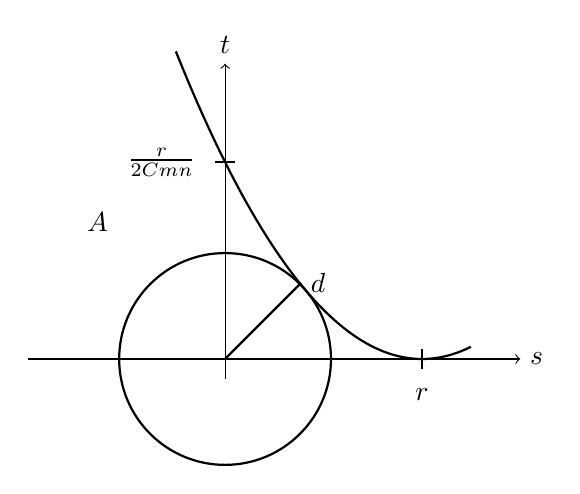
\begin{tikzpicture}[scale=2.5]
    % Draw the circle centered at (0,0) with radius 0.538
    \draw[thick,black] (0,0) circle[radius=0.538];
    
    % Draw the parabola y = (1-x)^2
    \draw[thick,black,domain=-0.25:1.25,samples=100] 
        plot ({\x}, {(1-\x)^2});
    
    \node[black,anchor=south west] at (-0.75, 0.60) {$A$};
    
    % Draw the axes
    \draw[->] (-1,0) -- (1.5,0) node[right] {$s$};
    \draw[->] (0,-0.1) -- (0,1.5) node[above] {$t$};
    
    % Draw the segment from (0,0) to (sqrt{0.538/2}, sqrt{0.538/2})
    \draw[thick,black] (0,0) -- (sqrt{0.538/1.9},sqrt{0.538/1.9});
    \node at (sqrt{0.538/1.9},sqrt{0.538/1.9}) [right] {$d$};
    
    % Draw the ticks
    \draw[thick] (1, 0.05) -- (1, -0.05); % Tick at (1, 0)
    \node at (1, -0.1) [below] {$r$};    % Label for (1, 0)
    
    \draw[thick] (-0.05, 1) -- (0.05, 1); % Tick at (0, 1)
    \node at (-0.1, 1) [left] {$\frac{r}{2Cmn}$}; % Label for (0, 1)
    
\end{tikzpicture}
\end{center}
Choosing $l_1 = (n-1)\,\widetilde{r}$, it can be shown that, for $C>1/8$, we indeed have that $l_1<d$. The goal would therefore be to verify that $$\sqrt{l_1^2-s^2} < \frac{(r-s)^2}{2Crmn}$$ for every $|s|<l_1$, but this is implied by 
\begin{equation} \label{l1}
l_1 < \frac{(r-l_1)^2}{2Crmn}\; ,
\end{equation}
an inequality that holds true if and only if $C > 1/(4mn) \leq 1/8$.

Now, we will generalize this for the function $\widetilde{y}_h$ in \ref{maggiorante} with $h$ fixed. It is analytic in the region 
$$A = \left\{ (x,t) \in \mathbb{R}^n : t<\frac{(r-(x_1+\ldots +x_{n-1}))^2}{2Crmn} \right\} .$$
The structure of the problem remains the same, so, naturally, the definition of $d$ remains unchanged. The only aspect we need to take care of is that, in this situation, it will be necessary to choose $l_2 =\widetilde{r}$. 
Thus, we want to show that $$\mathcal{L}=\sqrt{l_2^2-(x_1^2+\ldots +x_{n-1}^2)} < \frac{(r-(x_1+\ldots +x_{n-1}))^2}{2Crmn}=\mathcal{R}$$
when $|x|=|(x_1,\ldots ,x_{n-1})|< l_2$. But this is implied by the inequality \ref{l1}, which we know to be true. We will prove it in two steps.
\begin{itemize}
\item It holds that $\mathcal{L}^2< l_2^2 \leq l_1^2$ for $|x|< l_2$.
\item It holds that $$\left(\frac{(r-l_1)^2}{2Crmn}\right)^2 \leq \min \left\{ \mathcal{R}^2 : |x|\leq l_2 \right\}< \mathcal{R}^2 \, \text{ for } \, |x|< l_2.$$
This is shown knowing that $$\max \left\{ x_1+\ldots +x_{n-1} : |x|\leq l_2\right\}= (n-1)\frac{l_2}{\sqrt{n-1}}\leq l_1$$ and showing that $r-(x_1+\ldots +x_{n-1})>0$ for $|x|\leq l_2$ with the triangle inequality.
\qedhere
\end{itemize}
\end{proof}

\noindent\rule[0.5ex]{\linewidth}{0.2pt}

A careful reader will surely wonder about the reason behind choosing a constant $C\geq 1/2$. Well, this issue arises from what was left open in the proof of Theorem \ref{teoquasilin}, namely the fact that the solution $\widetilde{y}$ is indeed dominating only if $|(x,\widetilde{y}(x,t))|< r$. This property is precisely guaranteed in a ball of radius $\widetilde{r}$. Let us see this with a proposition that, in addition to clarifying, completes the logical framework of the proofs.
\begin{namedtheorem}[Proposition]\label{prop}
The domination of $\widetilde{y}$ holds in $B_{\widetilde{r}}(0)$, i.e.
$$|(x,t)|<\widetilde{r} \implies |(x,\widetilde{y}(x,t))|=x_1^2 + \ldots + x_{n-1}^2 + m \, u^2(x_1 + \ldots + x_{n-1},t) < r^2$$
\end{namedtheorem}
\begin{proof}
For simplicity, we demonstrate that $$|(s,t)|< l=(n-1)\,\widetilde{r} \implies s^2 + m \, u^2(s,t) < r^2.$$ The generalization is trivial if we take inspiration from the proof of Theorem \ref{stimaraggio}. 
\newpage
Considering that $|t|,|s|<l<r$ and that $s^2+t^2<l^2=r/(8Cmn)$, we write the following chain of inequalities.
\begin{align*}
& s^2 + m \left[ \frac{r-s-\sqrt{(r-s)^2-2tCrmn}}{mn} \right]^2\\ 
&\leq s^2 + \frac{1}{mn^2} \left[ (r-s)^2 + |(r-s)^2-2tCrmn| \right] 
&\begin{system}
\left|s\right| < r \Rightarrow r-s > 0\\
 \sqrt{(r-s)^2 - 2t Cr mn} > 0 
\end{system}\\
&\leq s^2 + \frac{2}{mn^2} (r-s)^2 + \frac{2|t|Crmn}{mn^2} \\ 
&\leq l^2 + \frac{2}{mn^2} \left( r^2 + l^2 + 2rl \right) + \frac{2lCrmn}{mn^2} 
&\begin{system}
\left|s\right| < l \Rightarrow (r-s)^2 < (r+l)^2\\
\left|t\right| < l
\end{system}\\
&= \left( \frac{r}{8Cmn} \right)^2 + \frac{2r^2}{mn^2} \left[ 1+\frac{1}{(8Cmn)^2} + \frac{1}{4Cmn} + \frac{1}{8} \right] \\ 
&< r^2 \underbrace{\frac{2}{mn^2} \left[ \frac{r}{8} + \frac{1}{(8C)^2 mn^2} + \frac{r}{(8Cmn)} + \frac{r}{4Cmn} + \frac{1}{8} \right]}_{<1} < r^2 \\ 
\end{align*}
In particular, the last statement holds because
\begin{align*}
n \geq 2 \Rightarrow \frac{2}{mn^2} \left(\ldots\right) 
&\leq \frac{1}{2} \left(\frac{9}{8} + \frac{2}{(8C)^2} + \frac{1}{8C}\right) \\ 
& \leq \frac{3}{16} \left(3 + \frac{1}{C}\right) < 1 & \Leftarrow C \geq \frac{1}{2} 
\end{align*}
\end{proof}



\newpage
\section{EDP in Normal Form}
Now we will utilize the results from the previous section to generalize that result to the case of an equation in normal form. To do this, it is sufficient to state and prove the following theorem.
\begin{theorem}\label{teonorm}
The following two problems are equivalent
\begin{align*}
\text{non-linear: }&
\begin{cases}
D_{t}^k u = G(x,t, D^\alpha_x D^j_t u) & |\alpha |+ j \leq k, \, j<k \\ 
D_t^ju = \phi_j & \text{ on } \Gamma_0, \, j<k 
\end{cases} \\ 
\text{quasi-linear: }&
\begin{cases}
D_t \, y = \sum\limits_{i=1}^{n-1} A_i(x,y)D_{x_i}y+B(x,y) \; \\ 
y=0 \quad \text{ on } \Gamma_0 
\end{cases}
\end{align*}
\end{theorem}

\begin{proof}
The reasoning is divided into three steps:
\begin{enumerate}
\item We construct the system such that $y_{\alpha j}= D^\alpha_x D^j_t u$. \\ 
Then, the matrices $A_i$ and $B$ can be obtained from the expressions
\begin{align*}
D_t y_{\alpha j} =& y_{\alpha (j+1)} & |\alpha| + j < k \\ 
D_t y_{\alpha j} =& D_{x_l} y_{(\alpha-e_l)(j+1)} & |\alpha| + j = k, \; j < k \\ 
D_t y_{0k} =& D_tG + \sum_{|\alpha|+j < k} D_{y_{\alpha j}}G y_{\alpha (j+1)} \\ 
& + \sum_{|\alpha|+j = k, \; j < k} D_{y_{\alpha j}} G D_{x_l} y_{(\alpha-e_l)(j+1)}
\end{align*}
where $l(\alpha)=\min\{ l:\alpha_l\neq 0 \}$, and the Cauchy data will be
\begin{align*}
y_{\alpha j}(x, 0) = & D_x^{\alpha} \phi_j(x) & j < k \\ 
y_{0k}(x, 0) = & G\left( x, 0, D_x^{\alpha} \phi_j(x) \right) & \lvert \alpha \rvert + j \leq k, \; j < k 
\end{align*}
\item We remove the conditions $\phi$, redefining $y(x,t)\leftarrow y(x,t)-\phi (x)$.
\item We eliminate the dependence on $t$, adding the variable $y^0=t$, together with the equation $D_t y^0=1$ and the data $y^0(x,0)=0$.
\end{enumerate}
We conclude by stating that, obviously, if $u$ is a solution of the problem in normal form, the $y_{\alpha j}$ will be solutions of the newly constructed problem. However, to demonstrate that $y_{(0,\ldots,0)}$ (solution of the latter) is also a solution of the problem in normal form, various calculations are necessary, which can be found in detail in \cite[cap.1]{Folland}.
\end{proof}

\begin{remark}
There are three aspects, which also emerge from the proof, that are worth briefly reflecting upon:
\begin{itemize}
\item Bringing together the considerations made at the beginning of the chapter and the theorems \ref{teoquasilin} and \ref{teonorm}, the CKT follows immediately;
\item The estimate of the radius of convergence continues to hold;
\item This equivalence theorem can be readily generalized to the case of a system in normal form.
\end{itemize}
\end{remark}

%\chapter{Esempi}

Dopo aver visto il CKT nella sua forma più nota, concentriamo ora lo sguardo su tre esempi importanti che aiutano a inquadrare meglio i limiti di questo teorema e il ruolo che giocano le ipotesi.

Tale discussione risulta particolarmente di rilievo, poiché per molto tempo si ritenne ragionevole pensare che un'equazione differenziale con coefficienti piuttosto regolari, come ad esempio $C^\infty$, dovesse avere almeno una soluzione. Questo, però, oltre al caso di analiticità trattato dal CKT, in generale non accade.


\section{Esempio di Lewy}
Questo primo esempio è decisamente il più importante ed interessante tra quelli qui trattati, 
proprio perché permette di introdurre, in modo più rigoroso, il problema appena citato.

Nel 1957 Hans Lewy propose un semplice controesempio, volto a mostrare come l'ipotesi di \textbf{analiticità} nel teorema di 
Cauchy-Kowalevski fosse cruciale, portando un caso di un operatore differenziale lineare con coefficienti analitici che necessita della presenza di una forzante anch'essa analitica per possedere delle soluzioni almeno $C^1$.

\emergencystretch 3em
Ciò mostra come sia cruciale, non solo una discussione sulle condizioni sufficienti per l'esistenza di soluzioni locali, 
ma anche una sulle condizioni necessarie. Infatti, Hörmander, matematico che contribuì ampiamente alla teoria delle equazioni lineari, 
rispose all'emersione di questo problema proprio con delle condizioni necessarie per l'esistenza di soluzioni locali 
(e quindi anche globali!) per equazioni lineari, le quali ispirarono poi, a loro volta, il lavoro di Treves e Nirenberg volto 
alla ricerca di condizioni necessarie e sufficienti.

\newpage
Preliminarmente si riportano qui sotto gli enunciati di due teoremi che torneranno utili nella discussione:

\begin{namedtheorem}[Formula di Green in $\mathbb{C}$]
\hpth{
D \subseteq \mathbb{C} \text{ dominio regolare }\\
f:D \rightarrow \mathbb{C}\\
f \in H(\interior{D})
}
{\oint\limits_{\partial^+D}f(z)\,dz=2i\iint\limits_D\frac{\partial f}{\partial \overline{z}}(x+iy)\,dxdy}
\end{namedtheorem}

\begin{remark}
La definizione di dominio regolare non ci tornerà particolarmente utile, infatti ai nostri scopi è sufficiente sapere che una qualsiasi palla chiusa è regolare (questo verrà utilizzato nella dimostrazione del teorema \ref{Lewy}). Per una formalizzazione di questo concetto si veda \cite[cap.8]{FMS}, dove è presente una trattazione dell'analogo teorema in $\mathbb{R}^2$ che va sotto il nome di ``Formule di Gauss-Green'' e ``Formula di Stokes'', di quale la generalizzazione in $\mathbb{C}$ è immediata.
\end{remark}

\begin{namedtheorem}[Principio di riflessione di Schwarz]
\hpth{
D \subseteq \mathbb{C} \text{ dominio regolare e simmetrico rispetto a } \mathbb{R}\\
D \cap\ \mathbb{R} \text{ è un intervallo }\\
f:D \rightarrow \mathbb{C}\\
f(\mathbb{R} \cap D) \subseteq \mathbb{R}\\
f \in H(\interior{D})
}
{f(\overline{z})=\overline{f(z)} \quad \forall z \in \interior{D}}
\end{namedtheorem}

\begin{remark}
La definizione di insieme simmetrico rispetto a $\mathbb{R}$ è data in modo naturale: esso deve soddisfare la condizione $z \in D \implies \overline{z} \in D$.
\end{remark}

\noindent\rule[0.5ex]{\linewidth}{0.2pt}

Per entrare nel vivo dell'esempio, definiamo il seguente operatore:
$$L=D_x+iD_y-2i(x+iy)D_t$$
che ha dei coefficienti $C^\infty$ e il cui comportamento peculiare emerge dal teorema che enunciamo di seguito.

\begin{theorem}\label{Lewy}
\hpth{
f \text{ funzione continua a valori reali che dipende solo da } \; t\\
u\in C^1\;:\;Lu=f \text{ in un intorno dell'origine }
}
{f \text{ analitica in un intorno di } t=0}
\end{theorem}

\begin{proof}
Innanzitutto fissiamo un $R>0$ tale che $\{(x,y,t): x^2+y^2<R^2,|t|<R\}$ sia contenuto nell'intorno dell'origine delle ipotesi (ovviamente questo $R$ esiste sempre) e procediamo seguendo cinque passi.
\begin{enumerate}[1.]
\item
Definiamo la funzione: 
\begin{equation*}
V(t,s)=\int\limits_{\gamma_r}u(x,y,t) \, dz \quad \text{con} \quad
\begin{system}
t \in (-R,R)\\
r^2=s \in [0,R^2)\\
\gamma_r=\partial^+B_r(0,0)\\
z=x+iy
\end{system}
\end{equation*}
\item
Troviamo una relazione tra $V_s$ e $V_t$:
\begin{align*}
V&=i\iint\limits_{B_r(0,0)}(u_x+iu_y)(x,y,t) \, dx \, dy &\text{per formula di Green}\\
&=i\int_0^r \int_0^{2\pi} (u_x+iu_y)(\rho \cos \theta,\, \rho \sin \theta,\, t) \, \rho \,d\rho \, d\theta &\text{in coordinate polari}\\
V_r&=i\int_0^{2\pi} (u_x+iu_y)(\rho \cos \theta,\, \rho \sin \theta,\, t) \, r \, d\theta &\text{derivando}\\
&=\int\limits_{\gamma_r}(u_x+iu_y)(x,y,t) \, r \, \frac{dz}{z}\\
V_s&=\frac{1}{2r}V_r=\int\limits_{\gamma_r}(u_x+iu_y)(x,y,t) \, \frac{dz}{2z}\\
&=\int\limits_{\gamma_r}u_t(x,y,t) \, dz + \int\limits_{\gamma_r}f(t) \, \frac{dz}{2z} &\text{usando } Lu=f\\
&=iV_t + \pi i f(t) \numberthis \label{eq:4}
\end{align*}
\item
Definiamo le funzioni:
\begin{align*}
F(t)&=\int_{0}^{t} f(\tau) \, d\tau\\
U(t,s)&=V(t,s)+\pi F(t)\;.
\end{align*}
e osserviamo le seguenti proprietà di $U$, vista come funzione di $w=t+is$: 
\begin{itemize}
\item
si può verificare che soddisfa l'equazione di Cauchy-Riemann $U_t+iU_s=2U_{\overline{z}}=0$ utilizzando la relazione \eqref{eq:4},
\item
è olomorfa per $(s,t) \in (0,R^2) \times (-R,R)$ per la proprietà precedente,
\item
è continua per $(s,t) \in [0,R^2) \times (-R,R)$ perché lo è $V$,
\item
$U(0,t)=\pi F(t)$ per $t\in (-R,R)$, ovvero assume valori reali sull'asse reale.
\end{itemize}
\item
Possiamo ora prolungare analiticamente $U$ in un intorno dell'origine, infatti, 
date le proprietà appena osservate, valgono le ipotesi del principio di riflessione di Schwarz, che ci permette 
di definire $U$ per $s\in (-R^2,0)$ con la seguente formula: $$U(t,s)=\overline{U(t,-s)}.$$
\item
Concludiamo il ragionamento notando che, se il prolungamento di $U$ è analitico in un intorno dell'origine, lo deve essere anche $U(t,0)=\pi F(t)$ e anche $f=F'$. \qedhere
\end{enumerate}
\end{proof}

\textbf{Generalization.} The theorem we just discussed can actually be extended to an interesting generalization, and the idea is as follows: we aim to show that, despite the characteristic form of $L$ having no singular points, it is possible to choose a forcing term $F \in C^{\infty} (\mathbb{R}^3, \mathbb{R})$ such that, \textbf{everywhere}, the differential equation $Lu=F$ admits no solutions.

\begin{remark}
Given two matrix spaces $(X,d_X)$ and $(Y,d_Y)$, the notation $C(X,Y)$ with $k \in \mathbb{N} \cup \{\infty\}$ denotes the set of continuous functions of the type $h:X \rightarrow Y$. In the case where $X=\mathbb{R}^n$ and $Y=\mathbb{R}^m$, we will naturally use the notation $C^k(\mathbb{R}^n,\mathbb{R}^m)$ for $C^k$ functions.
\end{remark}

Before delving into the specifics of this second part of the discussion on Lewy's example, it is useful to recall three definitions:
\begin{definition}
A subset $D$ of a topological space $X$ is dense if for every open set $A \in X$, $D \cap A \neq \emptyset$.
\end{definition}
\begin{definition}
A subset $E$ of a metric space has no interior if $\interior{E}=\emptyset$.
\end{definition}
\begin{definition}
A topological space is called a "Baire space" if the countable union of any family of closed sets with empty interior has empty interior.
\end{definition}

The reason we have mentioned these concepts is that we are interested in a theorem, or rather a corollary, that allows us to develop an argument by contradiction when dealing with complete metric spaces. The following statements are provided.

\begin{namedtheorem}[Baire Category Theorem]\label{Baire}
\hpthth{
(X,d) \text{ complete metric space }\\
\{A_n\}_{n \in \mathbb{N}} \subseteq 2^X \text{ family of dense open sets in } X\\
\{E_n\}_{n \in \mathbb{N}} \subseteq 2^X \text{ family of closed sets with no interior }
}
{\bigcap\limits_{n \in \mathbb{N}} A_n \text{ is dense in } X}
{\bigcup\limits_{n \in \mathbb{N}} E_n \text{ has no interior }}
\end{namedtheorem}

\begin{remark}
This theorem shows that complete metric spaces are indeed Baire spaces under the topology induced by the metric. See \cite[Ch.10]{RF} for the proof and more details.
\end{remark}

\begin{namedtheorem}[Corollary (Baire's argument by contradiction)]\label{arg-Baire}
\hpth{
(X,d) \text{ complete metric space }\\
\{E_n\}_{n \in \mathbb{N}} \subseteq 2^X \text{ family of closed sets }\\
X=\bigcup\limits_{n \in \mathbb{N}} E_n
}
{\exists \, n \in N \text{ such that } \interior{E_n} \neq \emptyset}
\end{namedtheorem}

\begin{remark}
This statement is the contrapositive of the second claim of theorem \ref{Baire}, and, as we mentioned earlier, it can be used to derive a contradiction by exhibiting a complete metric space equal to the union of a family of closed sets with no interior.
\end{remark}

The second important result from functional analysis, which will play a crucial role in achieving the stated goal, is the Ascoli-Arzelà theorem: a "compactness" theorem, which replaces the Heine-Borel theorem in the search for a convergent subsequence in cases where the compactness property of the metric spaces is not known. In particular, we will use it to show that a certain set (whose structure will be understood later) is closed, by exploiting the uniform convergence property guaranteed by the theorem.

To fully understand the statement of this theorem, we recall two definitions along with it.
\begin{definition}
A sequence of functions $\{f_n:X\rightarrow\mathbb{R}\}_{n \in \mathbb{N}_0}$ is said to be uniformly bounded in $X$ if $\exists \, M\geq 0$ such that $|f_n|\leq M$ in $X$.
\end{definition}
\begin{definition}
A sequence of functions $\{f_n:X\rightarrow\mathbb{R}\}_{n \in \mathbb{N}_0}$ is said to be equicontinuous in $X$ if $\forall \varepsilon >0 \;\, \exists \, \delta >0$ such that $d(x,y)<\delta \implies \abs{f_n(x)-f_n(y)}<\varepsilon \quad \forall x,y \in X,\, \forall n \in \mathbb{N}_0$.
\end{definition}
\begin{namedtheorem}[Ascoli-Arzelà Theorem]
\hpth{
(X,d) \text{ complete metric space }\\
\{f_n:X\rightarrow\mathbb{R}\}_{n \in \mathbb{N}_0} \text{ sequence of functions }\\
\quad - \quad \text{uniformly continuous}\\
\quad - \quad \text{uniformly bounded}
}
{\exists \, f\in C(X,\mathbb{R}), n_k \text{ such that } f_{n_k}\rightarrow f \text{ uniformly }}
\end{namedtheorem}

After reviewing these tools, it is time to delve into the discussion, and we do so by outlining the reasoning to be followed step by step:
\begin{enumerate}
\item
We will shift the problem of theorem \ref{Lewy} to refer to a generic point $(x_0,y_0,t_0)$, using the function $g(x,y,t)=f(t-2xy_0+2x_0y)$ as a forcing term (lemma \ref{lemma-tr});
\item
We will construct a function $S_a \in C^\infty$ for each $a \in l^\infty$ (lemma \ref{lemma-serie});
\item
We will build sets $E_{j,n} \subseteq l^\infty$ that are closed and have no interior using $S_a$ and the Ascoli-Arzelà theorem (lemma \ref{lemma-e});
\item
We will conclude the proof of theorem \ref{Lewy2} by using the aforementioned lemmas to derive, through a contradiction argument, the equality $l^\infty = \bigcup E_{j,n}$, which allows us to apply Baire's argument.
\end{enumerate}

Now we will detail the steps just outlined with statements and proofs.

\newpage
\begin{lemma}\label{lemma-tr}
\hpth{
F \in C^\infty(\mathbb{R},\mathbb{R})\\
(x_0,y_0,t_0)\in \mathbb{R}^3\\
u\in C^1\;:\;Lu(x,y,t)=F'(t-2xy_0+2x_0y) \text{ in a neighborhood of } (x_0,y_0,t_0)\\
}
{F \text{ and } F' \text{ are analytic in a neighborhood of } t=t_0}
\end{lemma}

\begin{proof}
By exploiting the invariance of the operator $L$ with respect to $$T(x,y,t)=(x+x_0,y+y_0,t+t_0+2xy_0-2x_0y),$$ i.e., the validity of the identity (easy to verify) $L(u \,\circ\, T)=(Lu) \circ T$, we deduce that, if $u$ is a solution to the equation in the hypothesis, it also holds in a neighborhood of the origin:
\begin{equation}\label{eq:10}
L(u \circ T)(x,y,t)=f(t+t_0) \text{ with } f=F'.
\end{equation}
Clearly, $u \circ T \in C^1$, and $g(t)=f(t+t_0)$ satisfies the conditions of theorem \ref{Lewy}, so by applying it to the second equation, the thesis is proved.
\end{proof}
\begin{remark}
The analyticity of $F$ follows from the last step in the proof of theorem \ref{Lewy}, considering that it takes the form $F(t)=\int_{0}^{t} f(\tau)+c$ with $c\in \mathbb{R}$.
\end{remark}
\begin{remark}
Equation \eqref{eq:10} holds in a neighborhood of the origin because the operator $T$ makes $\mathbb{R}^3$ a group, generally known as the Heisenberg group, and in this context, it acts like a translation.
\end{remark}


\begin{lemma} \label{lemma-serie}
\hpthth{
\{(x_j,y_j,t_j)\}_{j=1}^{\infty} \text{ dense in } \mathbb{R}^3\\ \label{eq:8} \numberthis 
c_j=2^{-j}e^{-\rho_j} \text{ with } \rho_j=|x_j|+|y_j| \quad \forall j \in \mathbb{N}_0\\
a=\{a_n\}_{n=1}^{\infty} \in l^{\infty}\\
F \in C^{\infty} (\mathbb{R},\mathbb{R}) \text{ periodic and non-analytic }\\
f_j(x,y,t)=F'(t+2xy_j-2x_jy)
}
{S_a=\sum_{j=1}^{\infty} a_jc_jf_j \text{ converges uniformly in } \mathbb{R}^3}
{\text{the same holds for the formal derivatives } D^{\alpha}S_a=\sum_{i=1}^{\infty} a_jc_jD^{\alpha}f_j}
\end{lemma}

\begin{remark}
Naturally, $S_a$ is a $C^\infty$ function.
\end{remark}

\newpage
\begin{proof}
Since $F$ is $C^\infty$ and periodic, we define ${M_k=\sup_t\abs{F^{(k)}(t)} \in \mathbb{R}}$ for every $k \in \mathbb{N}.$ This allows us to write, for each multi-index $\alpha$ and $j\in \mathbb{N}_0$, the following inequalities:
\begin{align*}
|a_jc_jD^{\alpha}f_j| &\leq \norm{a}_\infty \, 2^{-j} \, e^{-\rho_j} \, M_{| \alpha |+1} \, \rho_j^{| \alpha |} \\
&\leq \norm{a}_\infty \, 2^{-j} \, M_{| \alpha |+1} \left(\frac{| \alpha |}{e}\right)^{| \alpha |}& \text{ because } \max\limits_{x \geq 0}\frac{x^{| \alpha |}}{e^x} = \left(\frac{| \alpha |}{e}\right)^{| \alpha |} \label{eq:5}\numberthis
\end{align*}
$D^\alpha S_a$ converges absolutely, and therefore also uniformly, as the series $$\sum_{j=1}^{\infty} \sup\limits_{\mathbb{R}^3} |a_jc_j D^{\alpha} f_j|$$ has a general term that is less than or equal to the right-hand side of inequality \eqref{eq:5}, whose corresponding numerical series is obviously convergent.
\end{proof}

\begin{remark}
Before continuing, let's briefly pause on two noteworthy points:
\begin{itemize}
\item
$l^{\infty}$ is a Banach space when equipped with the norm: $\norm{b}_\infty=\sup_n|b_n|$ for every $b \in l^{\infty}$;
\item
there exists a function $f$ with the properties mentioned in the hypotheses: for instance, the function $$F(x)=\sum_{n=1}^\infty\frac{\cos(n!\,x)}{(n!)^n}$$ is defined by a pointwise convergent series and is $C^{\infty}(\mathbb{R},\mathbb{R})$. Additionally, it is periodic with period $2\pi$ and can be shown not to be analytic at any point $x\in\mathbb{R}$. For more on this, see problem 4 in \cite[cap.3]{John}.
\end{itemize}
\end{remark}
\textbf{Notation.} $A_{j,n} = B_{n^{-1/2}}(x_i,y_i,t_i)$ where $(x_i,y_i,t_i)$ are the points in the hypotheses of lemma \ref{lemma-serie}.
\begin{lemma}\label{lemma-e}
\hpth{
\text{Same hypotheses as lemma \ref{lemma-serie}}\\
\{E_{j,n}\}_{j,n \in \mathbb{N}_0} \subseteq l^{\infty} \text{ such that } \\ 
a \in E_{j,n} \text{ if and only if } \exists \, u \in C^1(A_{j,n}) \text{ such that }\\
\quad - \quad Lu=S_a \text{ in } A_{j,n}\\
\quad - \quad u(x_j,y_j,t_j)=0 \numberthis \label{eq:9} \\ 
\quad - \quad |D^{\alpha}u| \leq n \text{ for } | \alpha | \leq 1 \text{ in } A_{j,n} \\ 
\quad - \quad |D^{\alpha}u(v) - D^{\alpha}u(w)| \leq n |v-w|^{1/n} \text{ for }
\begin{system}
| \alpha | = 1\\
v,w \in A_{j,n}
\end{system}
}
{\{E_{j,n}\} \text{ are closed and nowhere dense sets}}
\end{lemma}

\newpage
\begin{proof}
We will prove the two properties separately.
\begin{enumerate}
\item
Regarding the property of closure, we want to show that if $\{a^k\}\subseteq E_{j,n}$ is such that $a^k \xrightarrow{l^\infty} a$, then $a \in E_{j,n}$. This, in turn, reduces to showing the existence of a function $u$ with the properties in \eqref{eq:9}.

We immediately deduce that $S_{a^k} \rightarrow S_a$ uniformly, since $\abs{S_a - S_{a^k}} \leq M_1 \norm{a-a^k}$ from \eqref{eq:5} with $\alpha = 0$. Additionally, due to the hypotheses on $a^k$, there exists a function $u_k$ that solves the equation $Lu_k=S_{a^k}$ and satisfies the other properties in \eqref{eq:9}. Due to these latter properties, $u_k$ satisfies the hypotheses of the Ascoli-Arzelà theorem with $X=A_{j,n}$, so for some $u$ it holds that $u_{k_h} \rightarrow u \text{ uniformly }$.

In particular, exploiting the fact that $L$ is a first-order operator, it is easy to deduce that $Lu=S_a$ in $A_{j,n}$ since
\begin{align*}
Lu_{k_h}& \rightarrow Lu &\text{ uniformly for the properties of } u_k\\
\lVert \quad &  &\\
S_{a^{k_h}}& \rightarrow S_a &\text{ uniformly }
\end{align*}
and that $u$ inherits all other properties in \eqref{eq:9} from $u_k$ due to uniform convergence.
 
\item
Finally, we will show that $\interior{E}_{j,n}=\emptyset$ by reasoning by contradiction. Thus, suppose there exists a sequence $a$ inside $\interior{E}_{j,n}$. Then, by defining
$$\delta_j = \frac{1}{c_j} \mathds{1}_{\{j\}} \in l^\infty,$$
we observe that there exists a $\theta \in \mathbb{R}$ small enough such that $a'=a+\theta \delta_j \in E_{j,n}$.
Now, let $u$ and $u'$ be the solutions to $Lu=S_a$ and $Lu=S_{a'}$ respectively, satisfying the properties in \eqref{eq:9}, and let
$$u''=\frac{u'-u}{\theta}.$$ 
Clearly, $u'' \in C^1$; moreover, using the linearity of $L$ and the definition of the series $S$, it is immediate to see that the relation $$Lu''=S_{\delta_j}=f_j$$ holds. However, this contradicts lemma \ref{lemma-tr} (whose hypotheses are all satisfied), since $F$ is not analytic. 
\end{enumerate}
\end{proof}


\newpage
\begin{theorem}\label{Lewy2}
\hpth{
A \subseteq \mathbb{R}^3 \text{ open }\\
}
{
\exists \, F \in C^{\infty}(\mathbb{R}^3,\mathbb{R}) \; : \; \nexists \, u \in C^1(A,\mathbb{R}) \text{ such that }
\begin{system}
Lu=F \text{ in } A\\
u_x,\,u_y,\,u_t \text{ satisfy }\\
\text {the Hölder condition }
\end{system}
}
\end{theorem}

\begin{remark}
The conclusion naturally implies that there are no $C^k$ solutions either, for any $k \geq 1$, since $C^k \subseteq C^1$.
\end{remark}

\begin{proof}
By reasoning by contradiction, we conclude with the following three steps (of which the second deserves the most attention).
\begin{enumerate}
\item
$E_{j,n} \subseteq l^{\infty} $ for every $j,n \in \mathbb{N}_0$, of course.
\item
$a \in l^{\infty} \implies a \in E_{j,n}$ for some $j,n \in \mathbb{N}_0$ (which depend on $a$).

Assuming the thesis is false, we can assert that $\forall a \in l^\infty \; \exists \, A \in \mathbb{R}^3, \, u^* \in C^1(A,\mathbb{R})$ such that $Lu^*=S_a$ and that $u^*$ has first derivatives continuous according to Hölder in $A$.

Moreover, due to the density of the set of points in \eqref{eq:8}, there exists a $(x_j,y_j,t_j) \in A$, and since $A$ is open, there exists a $k$ (chosen large enough) such that $A_{j,k} \subseteq A$.

Now consider the function $u=u^*-u^*(x_j,y_j,t_j)$, so that $u$ retains the properties of $u^*$, but at the same time satisfies the condition $u(x_j,y_j,t_j)$ as required in one of the properties in \eqref{eq:9}.

Finally, it is clear that, since the first derivatives of $u$ are continuous according to Hölder, there exists an $m$ large enough such that the remaining conditions in \eqref{eq:9} hold with $m$ instead of the subscript $n$, and then taking $n=\max\{k,m\}$, the implication is proven.

\item
From the first two steps, we conclude that $$l^{\infty}=\bigcup\limits_{j,n \in \mathbb{N}_0}E_{j,n},$$ but, therefore, since $l^{\infty}$ is a Banach space and due to the properties of the sets $E_{j,n}$, both the hypotheses of Corollary \ref{arg-Baire} and the negation of the thesis hold. This is absurd.
\end{enumerate}
\end{proof}


\newpage
\section{Kowalevski Example}

The example we now focus on is due to Kowalevski herself, and it was useful at the time to gain a deeper, more essential understanding of the importance, or rather the necessity, of assuming that the surface chosen to assign the Cauchy data is \textbf{non-characteristic} for the differential equation under observation. Moreover, it constitutes a counterexample to the conjecture proposed by Weierstrass, which suggested the possibility of defining analytic functions through differential equations.

All of this is mentioned in a letter addressed to Fuchs (a German mathematician from the University of Berlin) written by Weierstrass (who supervised Kowalevski's research), in which he requested the acceptance of Kowalevski’s doctoral thesis. The letter is fully reported in \cite[app.C]{Bio}.

Following in Kowalevski's footsteps, we consider the following Cauchy problem for the heat equation in one dimension:
\begin{align}
\label{eq:1}
u_t-u_{xx}&=0\\
\label{eq:2}
u(x,0)&=\frac{1}{1+x^2} \quad \forall \, x \in \mathbb{R}
\end{align}
\begin{remark}
In fact, the initial data actually chosen by Kowalevski during her research is $\frac{1}{1-x}$, but we have decided not to use it here for simplicity, avoiding some issues related to the singularity of the function while keeping the reasoning unchanged.
\end{remark}
Our goal is to prove that it admits no analytic solutions in a neighborhood of the origin.

\begin{enumerate}
\item
To begin, note that in this case, the surface on which the Cauchy data $(1.2)$ is assigned is
$\Gamma=\left\lbrace(x,t) \in \mathbb{R}^2:t=0\right\rbrace$. At every point, its normal vector is $(0,1)$ and, therefore, it is characteristic for the equation \eqref{eq:1}, since\footnote{see definition \ref{supcarlin}}
$$\sum_{|\alpha|=2}^{\;} a_\alpha \boldsymbol{\nu}^\alpha = a_{(2,0)}\boldsymbol{\nu}^{(2,0)} = 0. $$
\item
By contradiction, suppose we have a solution of the problem $u$ analytic in a neighborhood of the origin, that is:
$$u(x,t) = \sum_{\alpha = (\alpha_1, \alpha_2) }^{\;} c(\alpha) \, x^{\alpha_1} \, t ^{\alpha_2}, \quad
 c(\alpha) = \frac{D^\alpha u(0,0)}{\alpha!}$$
where $|(x,t)|<r$ for some $r>0$.
\item
We calculate the values of the coefficients $c(2n,0)$ $\forall n \in \mathbb{N}$.\\
To do this, we need to expand in power series, centered at the origin, the function of the Cauchy problem:
$$\frac{1}{1+x^2} = \frac{d}{dx}\arctan(x) = \frac{d}{dx}\sum_{n=0}^{\infty}\frac{(-1)^n}{2n+1} \, x^{2n+1} 
= \sum_{n=0}^{\infty}(-1)^n \, x^{2n} \quad \forall x \in \mathbb{R}.$$
From this series, we obtain the relations:
\begin{align*}
D_x^{2n}u(0,0) &= \frac{d^{2n}}{dx^{2n}} \left. \frac{1}{1+x^2}\right|_{x=0} = (-1)^n (2n)!\\
D_x^{2n+1}u(0,0) &= \frac{d^{2n+1}}{dx^{2n+1}} \left. \frac{1}{1+x^2} \right|_{x=0} = 0
\end{align*} 
from which we derive: $c(2n,0)=(-1)^n$ and $c(2n+1,0)=0$.
\item
We calculate the values of the coefficients $c(2n,n)$ and show that $c(2n,n) \xrightarrow{n\rightarrow\infty} +\infty$.\\
For this purpose, we use the equation \eqref{eq:1} to obtain the following relation between the coefficients:
\begin{equation} 
\label{eq:3}
c(\alpha_1,\alpha_2+1) = \frac{(\alpha_1+2)(\alpha_1+1)}{(\alpha_2+1)} \, c(\alpha_1+2,\alpha_2).
\end{equation}
And we use this as follows:
\begin{align*}
c(2n,n) &= \frac{(2n+2)(2n+1)}{n} \, c(2n+2,n-1)   &\eqref{eq:3}\quad\text{with} \quad 
\begin{system}
\alpha_1=2n\\
\alpha_2+1=n
\end{system}\\
 &= \ldots = \frac{(2n+2n)\cdots(2n+1)}{n!} \, c(2n+2n,0) &\text{\quad iterating over } n\\
 &= \frac{(4n)!}{(2n)! \, n!} (-1)^{2n} \\
 &\sim \frac{1}{\sqrt{\pi n}}\left(\frac{64n}{e}\right)^n \xrightarrow{n\rightarrow\infty} +\infty  &\text{using Stirling's formula}
\end{align*}
\item
We complete the reasoning by immediately observing that 
$$c(2n,n) \, x^{2n} \, t ^{n}\xrightarrow{n\rightarrow\infty} +\infty \quad \forall (x,t) \neq (0,0),$$ 
since this directly implies that the power series does not converge at any point other than the origin.
\end{enumerate}


\newpage
\section{Hadamard's Example}
The final example we address, due to Hadamard (1932), helps to understand an important limitation of the Cauchy-Kowalevski Theorem (CKT), namely the fact that it provides no control over the \textbf{relationship} between the Cauchy data and the form of the analytic solution: the problem may become unstable, meaning that small variations in the data may not correspond to small variations in the solution.

To observe this behavior, let us consider the following Cauchy problem for the two-dimensional Laplace equation as $n$ varies:
\begin{align*}
u_{xx}+u_{yy}&=0\\
u(x,0)&=0 \numberthis \label{eq:6}\\ 
u_y(x,0)&=n\sin(nx)e^{-\sqrt{n}} \quad \text{with} \quad n\in\mathbb{N}
\end{align*}

What we want to show is how, as $n$ increases, a blow-up of the solution $u_n$ of the problem \eqref{eq:6} occurs.
\begin{enumerate}[1.]
\item
The problem, as in the previous example, is assigned on $\Gamma=\left\lbrace(x,y) \in \mathbb{R}^2:y=0\right\rbrace$, which is naturally a non-characteristic surface for the Laplace equation (in fact, note that it is elliptic and thus possesses no characteristic surfaces).
\item
It is easy to verify that the function $u_n(x,y)=\sin(nx)\sinh(ny)e^{-\sqrt{n}}$ satisfies \eqref{eq:6} and that it is analytic, hence it is also the only possible solution with this property.
\item
Finally, we observe that $\sinh(ny)e^{-\sqrt{n}}\xrightarrow{n\rightarrow\infty} \infty$.
\end{enumerate}
As a conclusion to this discussion, let us consider the problem for ${n=\infty}$, that is, with data $u(x,0)=u_y(x,0)=0$, and we immediately notice that the only analytic solution is $u\equiv0$, which is naturally different from the asymptotic behavior of $u_n$. Therefore, we have just discovered that the solution does not continuously depend on the data.

Building on these considerations, Hadamard continued his studies, first defining the concept of well-posedness of a Cauchy problem\footnote{a Cauchy problem is well-posed if there exists a unique solution and it depends continuously on the initial data}, and then discovering that problems constructed with hyperbolic equations with constant coefficients always satisfy this condition in the class of $C^\infty$ functions.

%\include{chapters/6alternatives}
%\chapter{Conseguenze}
\section{Teorema di Holmgren}

\section{Altre applicazioni}
I. Ekeland

Cartan Kahler

4 (with Chiappori), "Aggregation and market demand: an exterior differential calculus viewpoint", Econometrica, 67 (1999), p. 1435-1458

This paper solves a basic problem in economic theory, which had remained open for thirty years, namely the characterization of market demand functions. The method of proof consists of reducing the problem to a system of nonlinear PDEs, for which convex solutions are sought. This is rewritten as an exterior differential system, and is solved by the Cartan-Kähler theorem, together with some algebraic manipulations to achieve convexity. The introduction of exterior differential calculus proved to be a breakthrough, and was the starting point of a long collaboration with P.A. Chiappori. We realized that the mathematical structure we had discovered in this problem was to be found also in one of the major problems of econometrics: given a group (a household, for instance), can one characterize and identify the preferences of each member if one observes only the collective demand ?. I am happy to say that this research program is now concluded, with the publication of two major papers [14] and [25] and a100-pages survey [28] which will probably turn into a book.

14: (with P.A. Chiappori) "The microeconomics of group behaviour: general characterization". Journal of Economic Theory, september 2006 , volume 130 (p.1 – 26)

25: (with P.A. Chiappori) "The microeconomics of group behaviour: Identification". Econometrica, 2005, 44 pages

28: (with P.A. Chiappori). "The mathematics and economics of aggregation". Foundations and Trends in Economic Theory, 2009

% BIBLIOGRAFIA
% PER FARLA FUNZIONARE: eseguire latex-bibtex-latex-latex
\addcontentsline{toc}{chapter}{Bibliography}
\nocite{*} % Inserire nella bibliografia anche le fonti non citate esplicitamente nel testo
\bibliographystyle{alpha} % We choose the "plain" reference style
\bibliography{bibliography} % Entries are in the refs.bib file

\end{document}